%!TeX root = molecular_dynamics
\documentclass[paper.tex]{subfiles}
\begin{document}

\section{Molecular dynamics simulation}
\
%\begin{multicols}{1}
%%%%%%%%%%%%%%%%%%%%%%%%%%%%%%%%%%%%%%%%%%%%%%%%


An illustrative - to ensure that there was nothing egregiously wrong with the Stokes drag calculation and to extract various. Certainly this has been done dozens of times in the past. For other reasons to play around with. ]\

\begin{figure}[H]
%	\makebox[\textwidth][c]{
	\centering
	\subfloat[Flower one.]{
	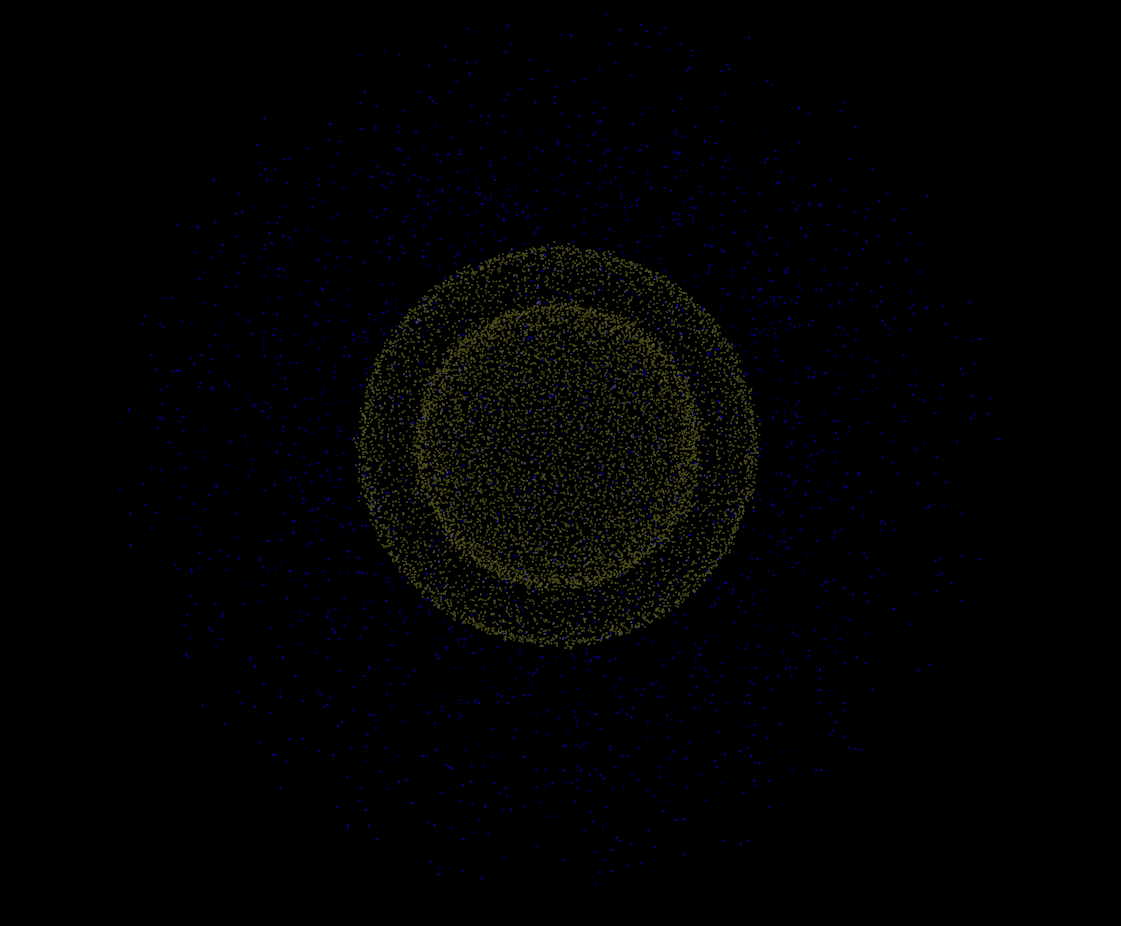
\includegraphics[width=0.4\textwidth]{Vescicle.png}

	}
	\hfill
	\subfloat[The observed spectrum]{
		\includesvg[width=0.4\textwidth]{spectrum}

	}
		\caption{Second.}
		
\end{figure}

These results are not in any way quantitative, nor do they truly suggest that the effect exists. Critical issues include the lack of deconvolution from the input impulse bandwidth. Lipid vesicle simulations with MARTINI force fields have yielded large-scale stiffness values which are orders of magnitude\cite{Determining2014} from those found experimentally; the speed of sound is also. 

A very large amount of tuning and comparison  to obtain any kind of meaningful  

the intitial transient must be deconvolved

Liposome wrapped with BUMPy\cite{BUMPy2018}. \footnote{Durrant's LipidWrapper are equally good options}. MARTINI 
coarse-grained 
lipid and water force field. Run with GROMACS (5?) on the GPU. A non-equlibrium simulation (very weak thermostat on lipid) with a thick layer of explicit water and then one monolayer of water with restraints (? N/m spring constant) and a strong thermostat () to crudely emulate a large thermal bath (an "open boundary"). This may not be a good way to do this.

molecular dynamics simulation of a lipid vescicle of 30 nm diameter. A mix of POPC and PUPI added to bring liposome charge to 
observed levels.

Rather than use standard eigenmode-style normal-mode methods (ProDy), Fourier analysis of the (lipid-only) trajectory was performed with TRAVIS\footnote{a really fantastic program. Clever user interface too!}, zero-padded at the end to obtain sufficient low-frequency bins with short simulations. The initial "spring Note the non-zero y-intercept. 

Computational pipeline available at \ghfile{biology/simulation/GROMACS/BUMPy_bilayer} \footnote{GALAXY or RENKU or some other, more repeatable and reproducible "pipeline manager" should have been used}. 

Polarizable water is usually required

Coarse-grained models of COVID with mechanically have recently been created; as of this writing the all-important nucleocapsid and RNA 



Interestingly, finite-element analysis appears to be a perfectly sensible approach to coarse-graining, just like might be done with a macro-scale structure.





It was originally expected that a large part of this work would be done in-silico, as we did not anticipate having access to suitable RF test equipment. 

Some time was spent attempting to set up a molecular dynamics toolchain capable of simulating an entire virus. 

Having an approximate simulation of the this technique would be useful for a number of reasons: 

We would have a better idea of the transferability to SARS, without wasting the time of experts with BSL-3/4 labs.

The impulse could be subjected to the same optimization as the RF feedback loop. A number of parameters (such as phase, polarization)



Coarse-graining also greatly increases the allowable timestep.

We also did not understand the *confined* part in the *confined* acoustic resonance.

Simulating the aggregate bose condensate wavefunction is well beyond us.


Both finite-element, molecular-dynamics, and stiffness-eigenvalue normal mode techniques have been used to great effect for this purpose. 


%\end{multicols}





\PRLsep{{\itshape Virus structural data }}

One extreme can be seen in 

Because CryoEM is sensitive to the 


\end{document}
